\section{Terminal mechanics}
\label{section:tty}
\epigraph{The tty layer is one of the very few pieces of kernel code that scares the hell out of me.}{Ingo Molnar\cite{molnarhell}}
You won't often need to deal with the gritty details of terminal access and
manipulation. It's still important to understand what's going on behind the
abstraction, especially for when things go wrong. As was made clear in
Chapters~\ref{sec:direct} and~\ref{sec:fullscreen}, Notcurses requires a
proper terminal definition and a handle to a terminal device, or initialization
will fail (NCURSES requires the same). With that said, the UNIX terminal layers
have never been, and are not now for the faint of heart\footnote{When Ingo
Molnar is scared, we all ought be scared.}. Extending back to the AT\&T dark
ages (and with at least three major distinct interfaces over the years, only unified
in 1997's SUS2), they are configured primarily through messy \texttt{ioctl}s and the
slightly-less-messy \texttt{termios} API.

More details than you probably want are available from Chapters 18 and 19 of \cite{apiue}
(general UNIX), Chapters 62 and 64 of~\cite{linuxprogramming} and Chapter 18
of~\cite{linuxdevicedrivers} (Linux), and Chapter 10 of~\cite{freebsddesign} (FreeBSD).

Modern workstations support a variety of physical and virtual terminal devices:
\begin{denseitemize}
\item{Honest-to-Bog serial terminals, probably using the RS-232\cite{rs232}
      protocol over a D-subminiature 25-pin (DB-25M) or 9-pin (DE-9M)
      connector (see Table~\ref{table:serial}).}
\item{Virtual consoles on text-based video, plus a keyboard.}
\item{Virtual framebuffer consoles on graphics-based video, plus a keyboard.} 
\item{Terminal emulators in a graphical environment, plus brokered input devices.}
\item{Pseudoterminals hooked up to network connections.}
\end{denseitemize}

\begin{table}[!htb]
  \centering
  \begin{tabular}{ |c|c|c|c|c| }
    \hline
    Signal & DB-25M & TIA-574 DE-9M & Yost 8P8C\cite{yost} & Originator \\
    \hline
    \hline
    Protective ground & 1 & x & x & x \\
    \hline
    Transmitted data & 2 & 3 & 3 & DTE \\
    \hline
    Received data & 3 & 2 & 6 & DCE \\
    \hline
    Request to send & 4 & 7 & 1 & DTE \\
    \hline
    Clear to send & 5 & 8 & 8 & DCE \\
    \hline
    Data set ready & 6 & 6 & 2 & DCE \\
    \hline
    Signal ground & 7 & 5 & 4, 5 & x \\
    \hline
    Carrier detect & 8 & 1 & 2 & DCE \\
    \hline
    Data terminal ready & 20 & 4 & 7 & DTE \\
    \hline
    Ring indicator & 22 & 9 & x & DCE \\
    \hline
  \end{tabular}
  \caption[RS-232/EIA-232 pin mappings]{RS-232/EIA-232 pins (DCE=Data circuit equipment, DTE=Data terminal equipment)}
  \label{table:serial}
\end{table}

On Linux, three kernel definitions form the core of the terminal abstraction
(the ``tty layer''). A \texttt{tty\_driver} function interface exists for each
tty implementation, and each has a different corresponding
major+minor device number pair. These implementations are enumerated in
\texttt{/proc/tty/drivers} (sample contents are listed in Table~\ref{table:procttydrivers}).
Line disciplines can be found in \texttt{/proc/tty/ldiscs}. The only line discipline
you're likely to encounter in a terminal context is \texttt{n\_tty}, the ``new tty''
discipline responsible for implementing ``cooked mode''\cite{essentialdrivers}.

\begin{figure}[!htb]
  \centering
  \includegraphics[width=.65\linewidth]{dot/tty-serial.png}
  \caption[A serial console, from hardware to userspace.]
  {A serial console, from hardware to userspace. Adapted from \cite{ttydemystified}.}
  \label{fig:ttysetups}
\end{figure}

POSIX.1-2017\cite{posix2017} §10.1 ``Directory Structure and Devices''
specifies three special files in the \texttt{/dev} directory, of which two are
related to the terminal/console system: \texttt{/dev/tty} is, within a process
context, a synonym for the controlling terminal associated with that process's
group (this can also be acquired with \texttt{tty(1)} or the POSIX C function
\texttt{ctermid(3)}\footnote{\texttt{/dev/tty} also uniquely supports the
\texttt{TIOCNOTTY} \texttt{ioctl(2)} for detaching a process from its
controlling terminal.}). The tty associated with an arbitrary file descriptor can
be retrieved with \texttt{ttyname\_r(3)}). \texttt{/dev/console} is a generic name for the current system console\footnote{Defined in \textit{ibid.} §3.392
``System Console'' as the device receiving messages sent by the \texttt{syslog()}
function. On Linux, it will also reproduce messages written to \texttt{/dev/kmsg}\cite{dmesg}.};
POSIX requires that the system console implement its ``General Terminal Interface'' (see
\textit{ibid.} §11). The standard console will by default be \path{/dev/tty0}, but this
can be changed with the \texttt{console=} kernel command line parameter, or with
an explicit \texttt{ConOut} UEFI variable (see §11.4 of \cite{uefi}). \texttt{/dev/tty0} is a special device on Linux linked to
the current virtual console (which might not be the system console). The
available system consoles can be found in \texttt{/proc/consoles}.

Initial \texttt{/dev/ttyN} devices are created internally by the kernel
(according to the value of \texttt{MAX\_NR\_CONSOLES}, by default 64) and set
up by \texttt{udev}. These are distinct devices, each usable by one virtual
console. Serial consoles show up as \texttt{/dev/ttySN}\cite{ttys4}. Each
virtual console gets a device at \texttt{/dev/vcsN} allowing access to the
glyph values of the console, a device at \texttt{/dev/vcsaN} allowing access to
the attributes at each cell, plus screen geometry, and a device at \texttt{/dev/vcsuN}
providing access to the Unicode values of each cell\cite{vcs4}. If a framebuffer console
is being used, these devices are prepared atop some framebuffer device \texttt{/dev/fbN} (see
Figure~\ref{fig:framebuffers}); these mappings can be managed with \texttt{con2fbmap(1)}.

\begin{figure}[!htb]
  \centering
  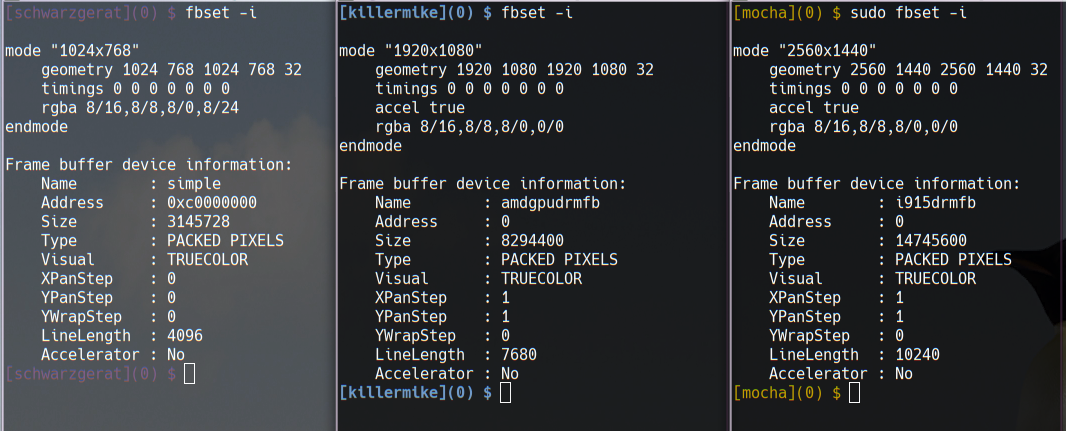
\includegraphics[width=.75\linewidth]{media/framebuffers.png}
  \caption{Three different Linux framebuffer implementations.}
  \label{fig:framebuffers}
\end{figure}

\begin{table}[!htb]
  \centering
  \begin{tabular}{ |c|c|c|c|c|c| }
    \hline
    Name & Default node & Major & Minor & Type & sysfs \\
    \hline
    \hline
    /dev/tty & /dev/tty & 5 & 0 & system:/dev/tty & devices/virtual/tty/tty* \\
    \hline
    /dev/console & /dev/console & 5 & 1 & system:console & devices/virtual/tty/console \\
    \hline
    /dev/ptmx & /dev/ptmx & 5 & 2 & system & devices/virtual/tty/ptmx \\
    \hline
    /dev/vc/0 & /dev/vc/0 & 4 & 0 & system:vtmaster & x \\
    \hline
    usbserial & /dev/ttyUSB & 188 & 0--511 & serial & x \\
    \hline
    serial & /dev/ttyS & 4 & 64--95 & serial & x \\
    \hline
    rfcomm & /dev/rfcomm & 216 & 0--255 & serial & x \\
    \hline
    pty\_slave & /dev/pts & 136 & 0--1048575 & pty:slave & x \\
    \hline
    pty\_master & /dev/ptm & 128 & 0--1048575 & pty:master & x \\
    \hline
    unknown & /dev/tty & 4 & 1--63 & console & devices/virtual/tty/console \\
    \hline
  \end{tabular}
  \caption[Expanded contents of \texttt{/proc/tty/drivers}]{Extended content of a sample \texttt{/proc/tty/drivers}\\
    (5.5.6 kernel. \texttt{sysfs} information has been added)}
  \label{table:procttydrivers}
\end{table}

The various termios flags allow very fine control of the kernel state associated
with a given terminal. It is possible to mix flag settings arbitrarily, but three
modes are common, and have their own nomenclature:
\begin{denseitemize}
\item{\textbf{Canonical mode, aka cooked mode:}   The terminal driver buffers input until a newline is entered, while echoing
    it to the screen. Ctrl+C is mapped to \texttt{SIGINT}, Ctrl+\textbackslash\ is
    mapped to \texttt{SIGQUIT}, and Ctrl+Z is mapped to \texttt{SIGTSTP}.
    Buffered input is flushed when these signals are sent. The default mode.}
\item{\textbf{Cbreak mode:} Line buffering is disabled, as is the processing
  of erase/kill characters. Interrupt and flow control translation is unaffected.
Sometimes referred to as \textit{rare mode}. This mode allows processing of input
without waiting for a newline character, while retaining e.g. Ctrl+C.}
\item{\textbf{Raw mode:} Interrupt and flow control translation is also disabled.
  This allows all keyboard input to be processed without preprocessing by the
  line discipline, but e.g. Ctrl+C behavior is lost, and (if desired) must be
  emulated in user space.}
\end{denseitemize}

\begin{figure}[!htb]
  \centering
  \includegraphics[width=.85\linewidth]{dot/tty-vesafb.png}
  \caption[VESA + USB virtual console, from hardware to userspace.]
  {VESA + USB virtual console, from hardware to userspace. Adapted from \cite{ttydemystified}.}
  \label{fig:vesasetups}
\end{figure}

In addition to these physically-backed devices, ptys---pseudoterminal devices\cite{pty7}---exist
to support virtual teletype functionality, wherein a process plays the role
of hardware. Pseudoterminals\footnote{You might
 hear about both System V and BSD pseudoterminals. SUS standardized around
the System V form, known on Linux as ``UNIX 98''. This term refers to 1997's
SUSv2 ¯\textbackslash\_(ツ)\_/¯. Trash BSD ptys look like \texttt{/dev/ttyLN} and \texttt{/dev/ptyLN}.}
back most terminal instances, including GUI terminal emulators, network
services such as SSH, and multiplexers such as \texttt{screen}. A pty provides a
bidirectional channel between a \textit{master} and \textit{slave}, with the
slave presenting a classic terminal interface (i.e. writing a Ctrl+C to the
master side will (under the cooked or cbreak disciplines) result in
\texttt{SIGINT} being delivered to the foreground process group.

The details of Linux pseudoterminal pair creation can be found on the \texttt{pts(4)}\cite{pts4} man page.
\texttt{posix\_openpt(3)}\cite{posixopenpt3} opens the ``master clone device''
\path{/dev/ptmx}, receiving a file descriptor corresponding to the new PTM (pseudoterminal master).
A new PTS (pseudoterminal slave) is created in \path{/dev/pts/}
\footnote{\path{/dev/pts} is typically its own \texttt{devpts} filesystem on Linux.}, whose name can be discovered by
providing the PTM file descriptor to \texttt{ptsname\_r(3)}.%\cite{ptsname3}.
Opening this PTS requires use of the \texttt{grantpt(3)} and \texttt{unlockpt(3)} calls.
Once both sides have been opened, data freely flows between the PTM and PTS.

You generally shouldn't need to be mess with TTYs or PTYs yourself as an
application developer, but now you know what all that junk clogging up
your \path{/dev} is. Some day when you mess up your initramfs, and
you're getting an error message like ``\path{/dev/ptmx} does not exist you have
no chance to survive make your time'' you'll know you're missing the
master clone device, some small consolation as you hopelessly reboot\footnote{Pro tip:
should you ever need supply input to programs which refuse to read from pipes
(e.g. \texttt{passwd}), you can pump the input through a named pty.}.

\subsection{Terminals and the UNIX process model}
\label{sec:unixprocs}

Understanding how these devices---physical or virtual---end up connected to
actual processes requires understanding some basic details of the UNIX
process model\footnote{For a more complete description, consult Chapter 9
of \cite{apiue}.}. Recall the UNIX principle that ``everything is a file''. Generally---and
this is true for all terminal devices---devices will be \texttt{open(2)}ed
using their \path{/dev} nodes, and then operated upon as a typical file
descriptor. You're no doubt aware that UNIX programs traditionally start with
at least three file descriptors open: 0 for \texttt{stdin}, 1 for
\texttt{stdout}, and 2 for \texttt{stderr}. Recall further that file descriptors
are by default not closed across an \text{exec(2)} call that replaces one
process's code with another object.

Each process has a process ID (PID) unique to its PID namespace (see
\texttt{clone(2)}\cite{clone2}, particularly the \texttt{CLONE\_NEWPID} flag).
Each process is a member of a \textit{process group}, and each process group
has its own process group ID (PGID)\footnote{Both PIDs and PGIDs are represented using \texttt{pid\_t}.}.
This PGID is equal to the \textit{group leader}'s PID, and each process group
has one and only one leader. Signals can be addressed to a process group by
supplying the negative PGID to e.g. \texttt{kill(2)}; a signal sent to a group
will be delivered to all processes of that group. One of the most common
scenarios in which multiple processes are kept in a single group is a shell
pipeline (a \texttt{fork(2)}ing process will usually place independent children
into a new process group). This is the essential facility underlying job control
(placing a job into the background, etc.), explaining why backgrounding
applies to an entire pipeline. Processes may be moved between process groups,
but only within a \textit{session}.

All process groups (and thus all processes) are members of some session. Each
session has a session ID (SID)\footnote{This session ID isn't really its own
unique value---it's implied by the session leader process.}. This SID
is the same as the PID of its \textit{session leader}. A session might or might
not have a controlling terminal (daemons disconnect themselves from their
controlling terminal). Login sessions almost always do have a controlling
terminal: the tty on which \texttt{login} was running (for a cosole session),
or the pty opened at process creation (for e.g. SSH or \texttt{xterm}). The
process groups of a session are divided into a single \textit{foreground group}
and zero or more \textit{background groups}.

Figure~\ref{fig:termprocs} shows the terminal-connected processes on one of
my Linux workstations, with their PIDs, PPIDs (parent process IDs), PGIDs
and SIDs. \texttt{agetty} is listening on tty1, spawned by
\texttt{init} (process 1). Xorg is sitting on tty7, having been spawned by a
display manager (which is \textbf{not} itself connected to a terminal). The
\texttt{bash} at PID 41599 is the child of a \texttt{screen} process.
\texttt{bash} at PID 846497 is a child of \texttt{sshd}.

\begin{figure}[!htb]
  \centering
\begin{verbatim}
[killermike](0) $ ps  --ppid 2 --deselect o pid,ppid,pgid,sid,tty,comm  | grep -v ?
    PID    PPID    PGID     SID TT       COMMAND
  41599   41598   41599   41599 pts/1    bash
  41654   41599   41654   41599 pts/1    rtorrent main
 510181       1  510181  510181 tty1     agetty
 510609  510187  510609  510609 tty7     Xorg
 846497  846495  846497  846497 pts/0    bash
 851850  846497  851850  846497 pts/0    ps
 851851  846497  851850  846497 pts/0    grep
[killermike](0) $
\end{verbatim}
\caption{Terminal-connected processes on a Linux machine.}
\label{fig:termprocs}
\end{figure}

Sessions affect how signals from the terminal are distributed. \texttt{SIGINT}
and friends (signals generated due to the line discipline) are sent to the
foreground process group. Only the foreground process can read from the
terminal; if a background process attempts to do so, it is sent \texttt{SIGTTIN}, the default
handler of which is to stop. A stopped background process will receive
\texttt{SIGCONT} when brought into the foreground. Likewise, a background
process will be sent \texttt{SIGTTOU} if it attempts to write to the terminal
when the TOSTOP tty flag is valid, or attempts to reconfigure the terminal in
any way\cite{sigterminals}.

Finally, it's worth knowing how terminals get turned into login sessions. Under
\texttt{systemd-logind}\cite{logind}, \texttt{agetty} processes are launched
on demand (i.e.\ on first transition to the virtual console) on \texttt{ttyN}
through the value of \texttt{NAutoVTs}. Should you be so unfortunate as to
still be running SysVinit in 2020, ttys are configured in \path{/etc/inittab}\footnote{If you're one of those people who pine for SysVinit, your opinions are bad, and you should feel bad.}.
On FreeBSD, \path{/etc/ttys} plays a similar role\cite{fbsdttys5}. \texttt{getty},
\texttt{agetty} et al condition the line (if necessary), prompt for a login
name, and then invoke \texttt{login} or a similar program. \texttt{login} prompts
for a password (or \texttt{sshd} performs authentication by myriad means), and
if the user is authenticated, \texttt{exec(2)s} a login shell as a new session.
This login shell inherits the terminal file descriptors from parent processes,
and passes them (by default) to its children.

Environment variables are also inherited across process boundaries, and by the
time the login shell is run, the all-important \texttt{LANG} and \texttt{TERM}
variables ought have been set. \texttt{LANG} defaults are based off the contents
of \path{/etc/locale.conf}. \texttt{TERM} is generally set by the terminal emulator itself,
or by \texttt{getty} on the console, and it is always forwarded by ssh\footnote{There is an exception; ssh does not forward \texttt{TERM} when the \texttt{-T}
parameter explicitly inhibits pty allocation.}. It's critical to have a correct \texttt{TERM}
value, and misinformation on configuring it runs rampant. Besides the NCURSES FAQ\cite{ncursesfaq},
I find the nosh project's \texttt{TERM} page\cite{noshterm} to be an excellent
resource, along of course with the \texttt{term(7)} man page\cite{term7}. You
will likely want to manually ensure that \texttt{COLORTERM} is properly defined
for 24-bit TrueColor, assuming your terminal supports it.

\subsection{Control sequences ANSI and otherwise}
\label{sec:escapes}
Quite early on, various hardware terminals began adding vendor-specific control
sequences---special bit patterns which, when present in the output stream,
would have effects other than simple emission of control or graphic
characters\footnote{How early? The Baudot code of 1870 already had a ``Letter
shift'', and the Teletypesetter news wire code of 1928 introduced ``Shift
in`` and ``Shift out``. Pretty goddamned early, then.}. These first took the
form of ``shifters'', which substituted regions of the code set (and form the
basis of ISO 2022-style character set extension). With the advance of electric
displays, it became desirable to apply systematic changes to the basic
character set, and to more flexibly update the screen. The VT52 employed Bob
Bemer's ESC control character\cite{bemeresc} to introduce certain control
sequences, and by the time ANSI X3.41 rolled along in 1974 (to become ECMA-48 in
1976), it was reasonable to start all control sequences with ESC (having been
made an official part of ASCII by ANSI X3.4-1968). The VT100 maintained
compatibility with VT52-style escapes, but its 1970 User Guide already
admonished programmers that ``All new software should be designed around the
VT100's ANSI mode.''\cite{vt100}.

It is rare to encounter a terminal that implements no ANSI control sequences; I
doubt any system exists which implements all of them\footnote{There's some
crazy stuff in ECMA-48. ``Media copy''? ``Disable manual input''? Many things
are woefully underspecified}. Given the somewhat vague nature of ECMA-48 even
in its most recent (1991) edition\cite{ecma48}, it is unlikely that two
terminals ever implement it the exact same way. Even assuming an ANSI terminal,
it's thus critical to use a terminal abstraction library (notwithstanding some
people's well-meaning claims\cite{lexihale}); see the next section for more
information. Most of the useful ANSI sequences are prefixed by ESC[ (0x27
0x5B), the ``Control Sequence Initiator''. A selection of the ANSI control
sequences is listed in Table~\ref{table:escapes} (but they should always be
used through terminfo, as we'll see in a moment).

\begin{table}[!htb]
  \centering
  \begin{tabular}{|c|c|c|l|}
    \hline
    Sequence & Name & Termcap & Description \\
    \hline
    \hline
    c & RIS & rs1 & Reset to original state \\
    \hline
    \lbrack$n$A & CUU & cuu & Move up $n$ rows \\
    \hline
    \lbrack$n$B & CUD & cud & Move down $n$ rows \\
    \hline
    \lbrack$n$C & CUF & cuf & Move right $n$ columns \\
    \hline
    \lbrack$n$D & CUB & cub & Move left $n$ columns \\
    \hline
    \lbrack$val\ldots val$m & SGR & sgr & Set graphic rendition \\
    \hline
  \end{tabular}
  \caption[ANSI (actually ECMA-48) escape codes]{A few ANSI (ECMA-48) escape codes. All sequences follow an ESC.}
  \label{table:escapes}
\end{table}

Note that some escapes commonly misattributed to ANSI come instead from some
DEC extension. The Restore Saved Cursor (RCO) and Save Cursor Position (SCO)
escapes, for instance, show up all over the Internet as ANSI escape sequences,
but no trace of them can be found in ECMA-48:1991.

In a relic from teletypes, ISO 646, ISO 2022, and ECMA-35 described use of
non-destructive backspace to produce composed characters from spacing ones.
This had been eliminated by ISO 4873, ECMA-43, and ISO 8859.

\subsection{Terminfo}
\label{sec:terminfo}
While developing the editor \texttt{ex}, a precursor to the great \texttt{vi},
Bill Joy implemented for BSD a database and set of functions abstracting away
the differences between terminal emulators (inspired by similar capabilities of
MIT's Incompatible Timesharing System\cite{itspdp}).
The terminal abstraction layer was ready-made for release as the original termcap
in 1968 (Ken Arnold would a few years later genericize the cursor optimization
routines as the original BSD Curses\cite{arnold1977}). The termcap database
(\path{/etc/termcap}) is indexed by terminal type and two-letter property name,
and maps them to boolean, numeric, and string capabilities.

Termcap has a number of limitations, and its use in new programs is strongly
discouraged. In its place is recommended terminfo, a more powerful scheme
originally introduced as part of Mary Ann Horton's\footnote{Formerly known as Mark
Horton.} AT\&T curses\cite{horton1982}. Notcurses makes extensive use of terminfo,
drawing from it all escapes save RGB. The terminfo database and API are
specified in SUS, much like Curses (and indeed the libtinfo installed on most
Linux machines is shipped as part of NCURSES). The terminfo database can be
dumped with \texttt{infocmp(1)}, and specific properties can be queried with
\texttt{tput(1)}. \texttt{tset(1)}, \texttt{clear(1)}, and \texttt{reset(1)}
are usually wrappers around terminfo.

The \texttt{stty} tool accidentally duplicates some functionality of terminfo,
but it does not itself make use of terminfo. It is more accurate to describe
\texttt{stty} as a command-line interface to the termios routines
\texttt{tcgetattr()} and \texttt{tcsetattr()}. Dump all terminal attributes to
the screen with \texttt{stty -a}\footnote{Pro tip: \texttt{stty} generally works
  only on standard input\textellipsis but redirecting standard input from a
  \texttt{/dev} node works just fine (subject to permissions, of course).}.

\begin{figure}[!htb]
  \centering
  \includegraphics[width=.9\linewidth]{dot/fdsessions.png}
  \caption[Processes, sessions, PPIDs, and TTYs.]
  {Processes, sessions, PPIDs, and TTYs. Each grey box is a lineage of processes.
  Session IDs are listed. Columns are process names, PIDs, PPIDs, and open TTY.}
  \label{fig:fdsessions}
\end{figure}
